\documentclass[12pt]{beamer}
\usepackage[utf8]{inputenc}
\usetheme{PaloAlto}
\usepackage{graphicx}
\usepackage{booktabs}
\usepackage{amsthm}
\usepackage[english]{babel}
\logo{
\includegraphics[height=1cm]{logo.png}}
\title[Octave]{Introducción e Instalación de Octave}

\author{Anderson Daniel Grajales Alzate}
\institute[Universidad EAFIT]
{Análisis Numérico / Procesos Numéricos \\ % Your institution for the title page
	\medskip
	\textit{agrajal7@eafit.edu.co} % Your email address
	
}
\date{Febrero 7 de 2019}


\newtheorem{command}{Comandos}
\newtheorem{oper}{Operadores}
\newtheorem{prob}{Problema}
\newtheorem{sol}{Solución}

\begin{document}
	
	\begin{frame}
	\titlepage % Print the title page as the first slide
\end{frame}

\begin{frame}[allowframebreaks]{Contenidos}
\tableofcontents
\end{frame}


%   PRESENTATION SLIDES

\section{Introducción a Octave}

\subsection{Octave} %

\begin{frame}{Octave}
\begin{itemize}
	\item \text{GNU Octave} es un lenguaje de programación científica de alto nivel cuyo propósito principal es el trabajo con cómputos numéricos. 
	\item Provee una interfaz de línea de comandos para resolver problemas lineales y no lineales.
	\item Posee una gran cantidad de herramientas que permiten resolver problemas comunes del álgebra lineal, encontrar raíces de una función, integración y diferenciación de funciones, etc.
	\item Es un software libre.
	\item Es mayormente compatible con Matlab. 
\end{itemize}
\end{frame}

\section{Instalación}

\subsection{Windows}
\begin{frame}{Instalación en Windows}
\begin{itemize}
	\item Acceder a \href{https://www.gnu.org/software/octave/download.html}{https://www.gnu.org/software/octave/download.html}
	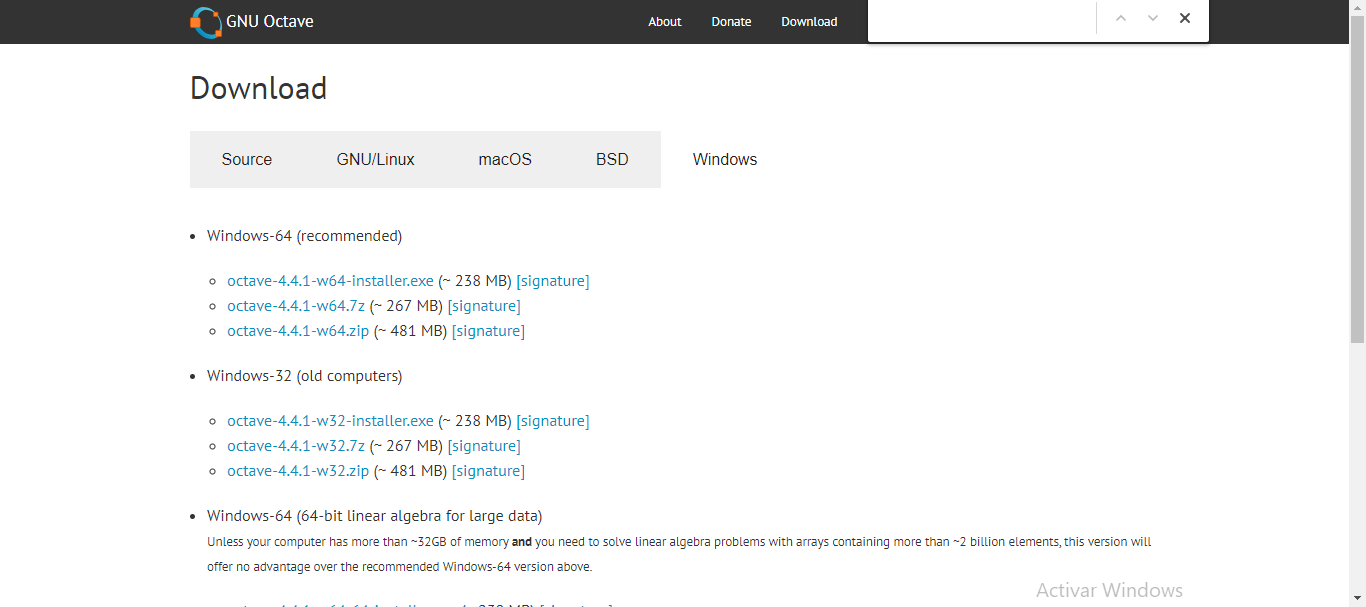
\includegraphics[scale=0.3]{imagen_octave}	
\end{itemize}
\end{frame}
\begin{frame}{Instalación en Windows}
\begin{itemize}
	\item Seleccionar la pestaña \textbf{Windows} \href{https://www.gnu.org/software/octave/download.html}{https://www.gnu.org/software/octave/download.html}
	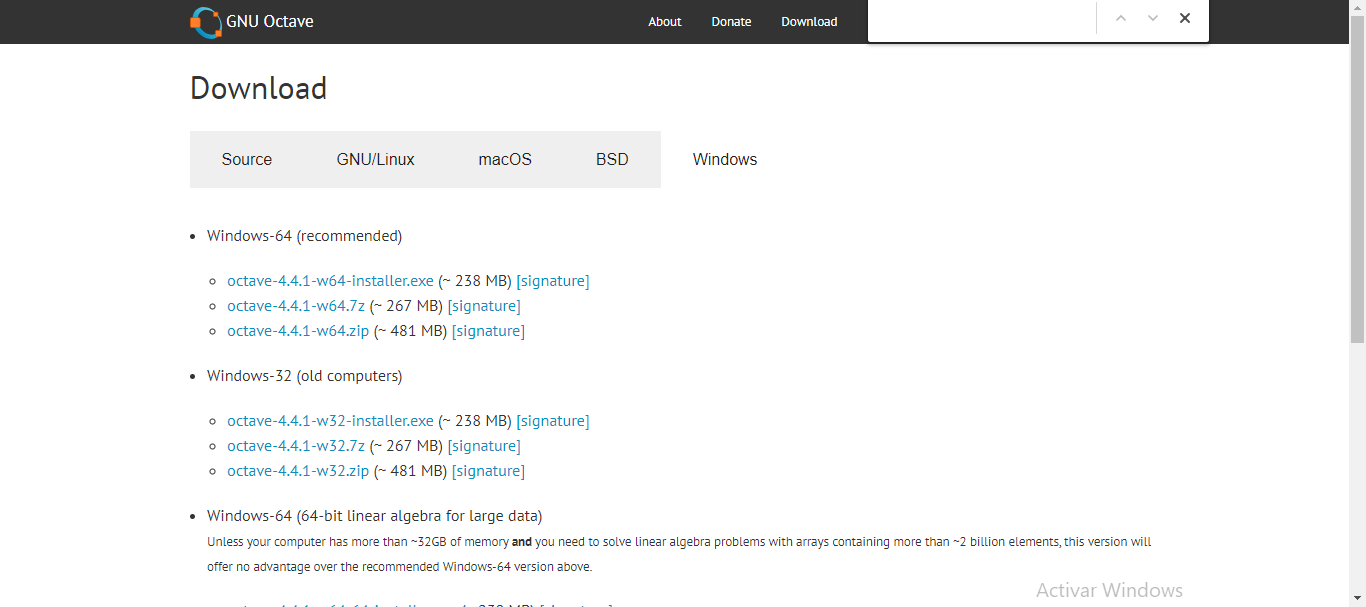
\includegraphics[scale=0.3]{imagen_octave}	
\end{itemize}
\end{frame}
\begin{frame}{Instalación en Windows}
\begin{itemize}
	\item Si tu sistema operativo es de 32-bits dar click en \textbf{octave-4.4.\textit{x}-w64-installer.exe}
	\item Si tu sistema operativo es de 64-bits dar click en \textbf{octave-4.4.\textit{x}-w32-installer.exe}
\end{itemize}
\end{frame}
\subsection{Linux/CentOS}
\begin{frame}{Instalación en Linux/CentOS}
\begin{command}
	\begin{itemize}
		\item sudo su
		\item yum install epel-release
		\item yum install octave
	\end{itemize}
\end{command}
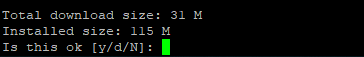
\includegraphics[height=1cm]{imagen_centos.png}
\end{frame}
\subsection{Linux/Ubuntu}
\begin{frame}{Instalación en Linux/Ubuntu}
\begin{command}
	\begin{itemize}
		\item sudo su
		\item apt-get install octave
	\end{itemize}
\end{command}
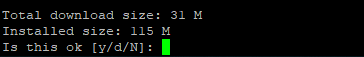
\includegraphics[height=1cm]{imagen_centos.png}
\end{frame}

\section{GUI Básica}
\subsection{GNU Octave CLI}
\begin{frame}{CLI}
Es una interfaz donde podemos ejecutar todas las funciones y comandos que nos provee GNU Octave.
\end{frame}
\begin{frame}{CLI}
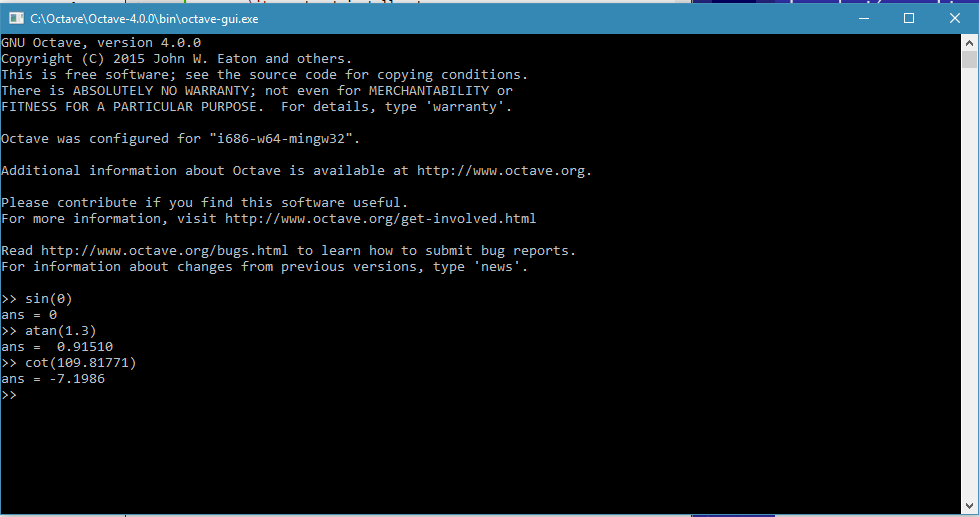
\includegraphics[width=270pt]{cli.png}
\end{frame}
\subsection{GNU Octave GUI}
\begin{frame}{GNU Octave GUI}
Al igual que en el CLI, en el GUI de GNU Octave, podemos ejecutar toas las funciones y comandos de Octave. Además, en el GUI tenemos una interfaz un poco más amigable y podemos crear \textit{Scripts} de manera sencilla con el editor que éste nos provee.
\end{frame}
\begin{frame}{GNU Octave GUI}
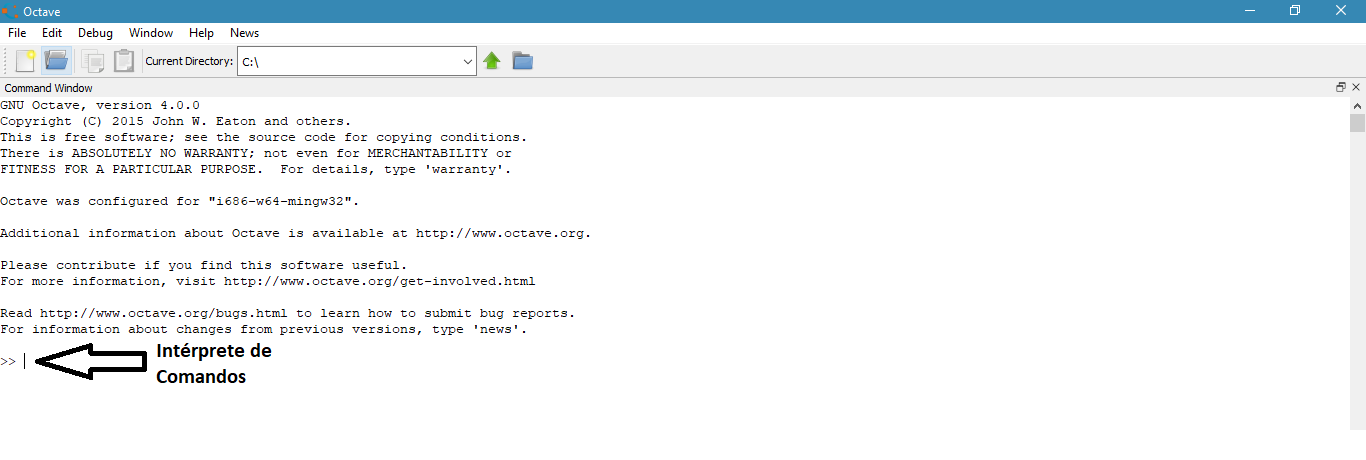
\includegraphics[width=270pt]{inter.png}
\end{frame}
\begin{frame}{GNU Octave GUI}
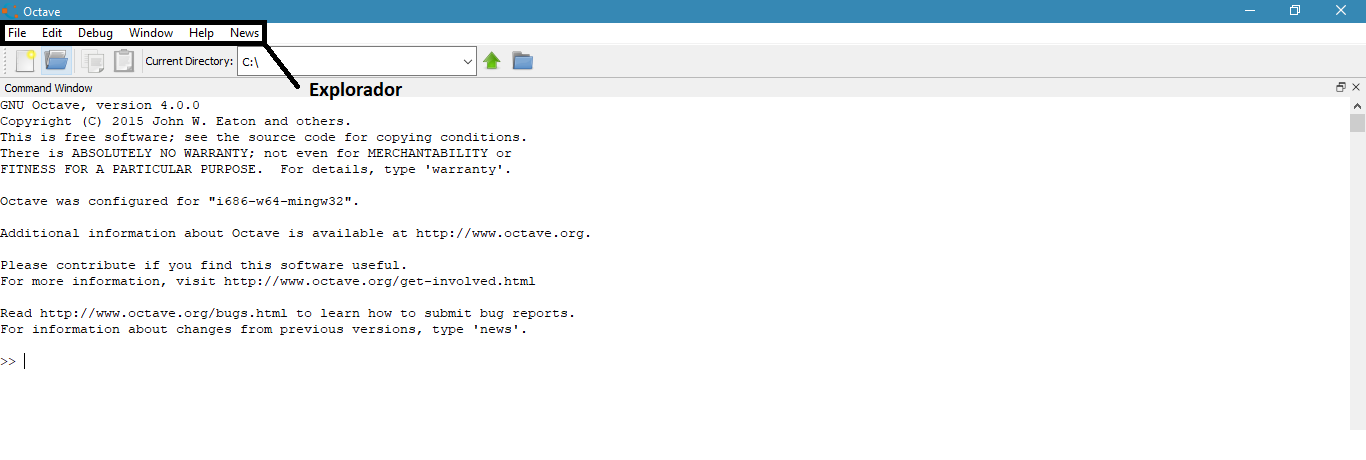
\includegraphics[width=270pt]{explor.png}
\end{frame}
\begin{frame}{GNU Octave GUI}
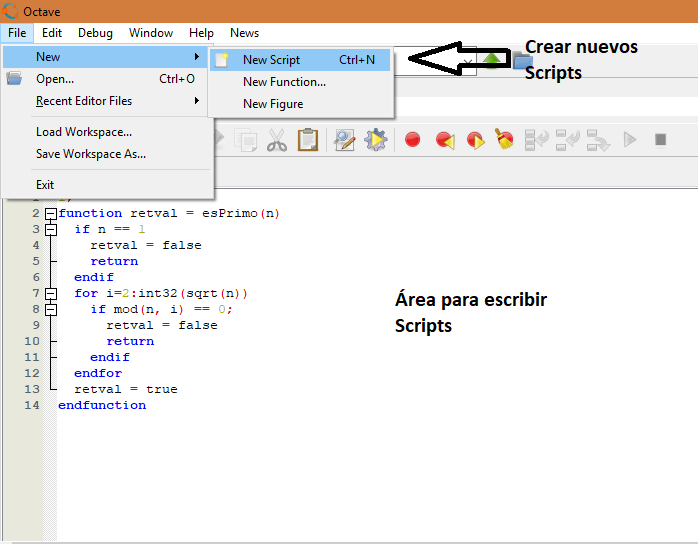
\includegraphics[width=270pt]{scripts.png}
\end{frame}
\section{Comandos Básicos}
\subsection{Operadores Básicos}
\begin{frame}{Operadores Básicos}
\begin{oper}
	\begin{itemize}
		\item / (División)
		\item * (Multiplicación)
		\item + (Suma)
		\item - (Resta)
		\item $mod(a, b)$ (Módulo)
		\item (\^\space\space $\mid$ ** ) (Potencia) 
	\end{itemize}
\end{oper}
\end{frame}

\subsection{Funciones Básicas}
\begin{frame}{Funciones Básicas}
GNU Octave cuenta con muchas funciones matemáticas que nos permiten resolver muchos problemas, entre éstas funciones están las siguientes:
\end{frame}
\begin{frame}{Funciones Básicas}
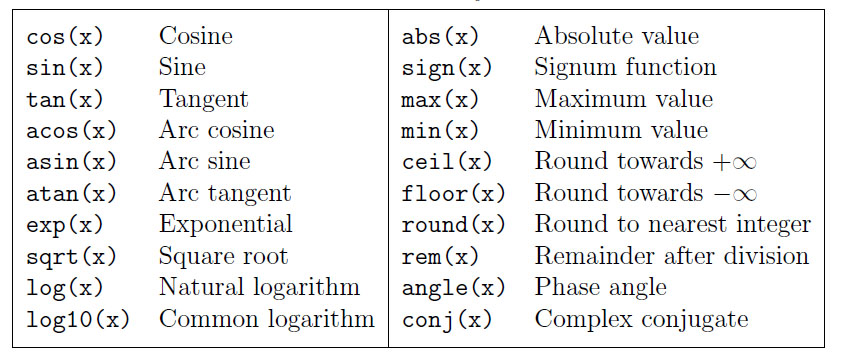
\includegraphics[width=270pt]{functions.jpg}
\end{frame}
\subsection{Vectores y Matrices}
\begin{frame}{Definición de Vectores y Matrices}
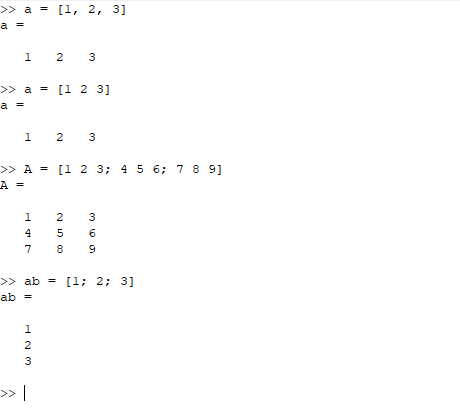
\includegraphics[height=220pt]{vectmat.png}
\end{frame}
\subsection{Álgebra Lineal}
\begin{frame}{Solución de Sistemas de Ecuaciones}
	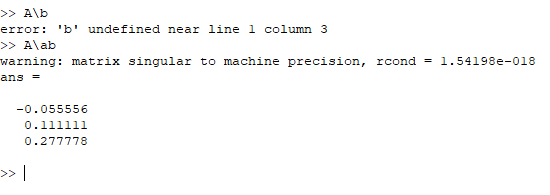
\includegraphics[]{sol.png}
\end{frame}
\section{Ejercicios}
\subsection{Ejercicio 1}
\begin{frame}{Ejercicio 1}
\begin{prob}
Determine los valores de $x_1, x_2$ y $x_3$ que satisfacen el siguiente sistema de ecuaciones.	
\begin{alignat*}{4}
2x_1 & {}+{} &  x_2 & {}+{} & 3x_3 & {}={} & 10 \\
x_1 & {}+{} &  x_2 & {}+{} &  x_3 & {}={} &  6 \\
x_1 & {}+{} & 3x_2 & {}+{} & 2x_3 & {}={} & 13
\end{alignat*}
\end{prob}
\end{frame}
\subsection{Solución 1}
\begin{frame}{Solución 1}
\begin{sol}
	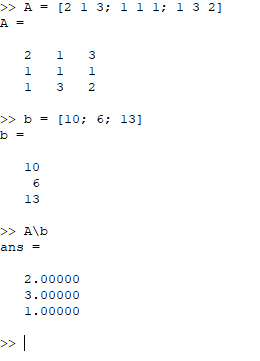
\includegraphics[height=180pt]{sol1.png}
\end{sol}
\end{frame}
\subsection{Ejercicio 2}
\begin{frame}{Ejercicio 2}
\begin{prob}
	La distancia del punto $(x_0, y_0)$ a la recta $ax + by + c = 0$ está dada por la ecuación:
	\[d = \frac{|a(x_0) + b(y_0) + c|}{\sqrt{a^2 + b^2}}\]
	Calcule la distancia de $(7, \frac{1}{2})$ a la recta $2x + 3y = 5$. 
\end{prob}
\end{frame}
\subsection{Solución 2}
\begin{frame}{Solución 2}
\begin{sol}
	 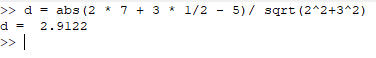
\includegraphics[width=270pt]{sol2.png}
\end{sol}
\end{frame}

\subsection{Ejercicio 3}
\begin{frame}{Ejercicio 3}
	\begin{prob}
		Para integrar una función $f(x)$ con la Fórmula de Simpson, se usa la expresión:
		\[
		\int_{a}^{b} {f(x) dx} \approx \frac{b - a}{6}\left(f(a) + 4f\left(\frac{a + b}{2}\right) + f(b)\right)
		\]
		Calcule la integral $\int_{0}^{4}{x^4 dx}$.
	\end{prob}
\end{frame}

\subsection{Solución 3}
\begin{frame}{Solución 3}
\begin{sol}
	 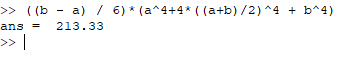
\includegraphics[width=270pt]{sol3.png}	
\end{sol}
\end{frame}
\section{Fin}
\subsection{Fin}
\begin{frame}{Fin}
	\centering \Huge
	\emph{Gracias}
\end{frame}

\end{document}